\documentclass[12pt]{thesis}
\bibliographystyle{unsrt}
%%% jdummy.def
%
\DeclareRelationFont{JY1}{mc}{it}{}{OT1}{cmr}{it}{}
\DeclareRelationFont{JT1}{mc}{it}{}{OT1}{cmr}{it}{}
\DeclareFontShape{JY1}{mc}{m}{it}{<5> <6> <7> <8> <9> <10> sgen*min
    <10.95><12><14.4><17.28><20.74><24.88> min10
    <-> min10}{}
\DeclareFontShape{JT1}{mc}{m}{it}{<5> <6> <7> <8> <9> <10> sgen*tmin
    <10.95><12><14.4><17.28><20.74><24.88> tmin10
    <-> tmin10}{}
\DeclareRelationFont{JY1}{mc}{sl}{}{OT1}{cmr}{sl}{}
\DeclareRelationFont{JT1}{mc}{sl}{}{OT1}{cmr}{sl}{}
\DeclareFontShape{JY1}{mc}{m}{sl}{<5> <6> <7> <8> <9> <10> sgen*min
    <10.95><12><14.4><17.28><20.74><24.88> min10
    <-> min10}{}
\DeclareFontShape{JT1}{mc}{m}{sl}{<5> <6> <7> <8> <9> <10> sgen*tmin
    <10.95><12><14.4><17.28><20.74><24.88> tmin10
    <-> tmin10}{}
\DeclareRelationFont{JY1}{mc}{sc}{}{OT1}{cmr}{sc}{}
\DeclareRelationFont{JT1}{mc}{sc}{}{OT1}{cmr}{sc}{}
\DeclareFontShape{JY1}{mc}{m}{sc}{<5> <6> <7> <8> <9> <10> sgen*min
    <10.95><12><14.4><17.28><20.74><24.88> min10
    <-> min10}{}
\DeclareFontShape{JT1}{mc}{m}{sc}{<5> <6> <7> <8> <9> <10> sgen*tmin
    <10.95><12><14.4><17.28><20.74><24.88> tmin10
    <-> tmin10}{}
\DeclareRelationFont{JY1}{gt}{it}{}{OT1}{cmbx}{it}{}
\DeclareRelationFont{JT1}{gt}{it}{}{OT1}{cmbx}{it}{}
\DeclareFontShape{JY1}{mc}{bx}{it}{<5> <6> <7> <8> <9> <10> sgen*goth
    <10.95><12><14.4><17.28><20.74><24.88> goth10
    <-> goth10}{}
\DeclareFontShape{JT1}{mc}{bx}{it}{<5> <6> <7> <8> <9> <10> sgen*tgoth
    <10.95><12><14.4><17.28><20.74><24.88> tgoth10
    <-> tgoth10}{}
\DeclareRelationFont{JY1}{gt}{sl}{}{OT1}{cmbx}{sl}{}
\DeclareRelationFont{JT1}{gt}{sl}{}{OT1}{cmbx}{sl}{}
\DeclareFontShape{JY1}{mc}{bx}{sl}{<5> <6> <7> <8> <9> <10> sgen*goth
    <10.95><12><14.4><17.28><20.74><24.88> goth10
    <-> goth10}{}
\DeclareFontShape{JT1}{mc}{bx}{sl}{<5> <6> <7> <8> <9> <10> sgen*tgoth
    <10.95><12><14.4><17.28><20.74><24.88> tgoth10
    <-> tgoth10}{}
\DeclareRelationFont{JY1}{gt}{sc}{}{OT1}{cmbx}{sc}{}
\DeclareRelationFont{JT1}{gt}{sc}{}{OT1}{cmbx}{sc}{}
\DeclareFontShape{JY1}{mc}{bx}{sc}{<5> <6> <7> <8> <9> <10> sgen*goth
    <10.95><12><14.4><17.28><20.74><24.88> goth10
    <-> goth10}{}
\DeclareFontShape{JT1}{mc}{bx}{sc}{<5> <6> <7> <8> <9> <10> sgen*tgoth
    <10.95><12><14.4><17.28><20.74><24.88> tgoth10
    <-> tgoth10}{}
\DeclareRelationFont{JY1}{gt}{it}{}{OT1}{cmr}{it}{}
\DeclareRelationFont{JT1}{gt}{it}{}{OT1}{cmr}{it}{}
\DeclareFontShape{JY1}{gt}{m}{it}{<5> <6> <7> <8> <9> <10> sgen*goth
    <10.95><12><14.4><17.28><20.74><24.88> goth10
    <-> goth10}{}
\DeclareFontShape{JT1}{gt}{m}{it}{<5> <6> <7> <8> <9> <10> sgen*tgoth
    <10.95><12><14.4><17.28><20.74><24.88> tgoth10
    <-> tgoth10}{}
\endinput
%%%% end of jdummy.def

 				% フォント関連のエラー対策(らしい)
\usepackage[dvipdfmx]{graphicx}
\usepackage{amsmath}			% math系
\usepackage{amssymb}			% math系
%\usepackage{float}				% 図表の挿入箇所を固定する[H]指定
\usepackage{cite}				% 参考文献
%\usepackage{url}				% 参考文献中のURL表記
\usepackage{algorithm}			% アルゴリズム環境
\usepackage{algorithmic}			% アルゴリズム環境
\usepackage{comment}			% コメントアウト環境
\usepackage{bm}					%太字形式のベクトル
\usepackage{amsthm}			%定理用?

\usepackage{breqn} %長い数式改行用

%%% 泉先生がコメントをつける用 %%%
\usepackage[normalem]{ulem}
\usepackage{color}
\newcommand{\Izumi}[1]{\textcolor{blue}{(#1)}}
\newcommand{\Izurep}[2]{\textcolor{red}{\sout{#1}}{\Izumi{#2}}}

%\headsep=1.4cm  %本文上にスペースを空けたい場合は 20mm にする

\newcommand{\CONGEST}{\textsf{CONGEST}}
\newcommand{\LOCAL}{\textsf{LOCAL}}

\newcommand{\Inp}{\mathit{in}}
\newcommand{\Out}{\mathit{out}}

% 定理環境
\usepackage{amsthm} %定理用
\theoremstyle{definition}
\newtheorem{theorem}{定理}[chapter]
\newtheorem{lemma}{補題}[chapter]
\newtheorem{definition}{定義}[chapter]
\newtheorem{fact}{事実}[chapter]
\newtheorem*{prf*}{証明}
%\renewcommand{\theproof}{}
%\newcommand{\qed}{\hfill$\square$\par}

%%%%%%%% ここから本体 %%%%%%%%%%%%%%%%%%%%%%%%

\begin{document}
\baselineskip=22pt
\pagestyle{empty}

% タイトル
%\gradyear{2020}
\papertitleJP{$k$-極大独立集合検証問題の \\ 分散計算複雑性}
\papertitleEN{Distributed Complexity of $k$-Maximal \\ Independent Set Verification}
\studentID{31414050}
\degree{master}
\program{cs}
\labo{片山・金}
\enteryear{2019}
\name{佐藤 僚祐}
\maketitle

% 目次
\pagestyle{myheadings}	% ページ番号を右上につける
\pagenumbering{roman}	% ページ番号をローマ数字で
\tableofcontents

\newpage

% 本文
\pagenumbering{arabic}	% ページ番号をアラビア数字で

\chapter{はじめに}

\section{研究背景}
分散グラフアルゴリズムとは,計算機を頂点,辺を通信リンクとみなしてネットワークをモデル化したグラフ上において,
そのネットワーク自身を入力として定義されるグラフアルゴリズム上の諸問題を解く枠組みである.分散アルゴリズムにおける
代表的なモデルのひとつとして{{\CONGEST}}モデルが存在する.{\CONGEST}モデルでは,
各ノードは同期ラウンドに従って実行され,メッセージ交換によって協調動作を行う.
各ノードは各ラウンドで(i)$O(\log n)$ビットのメッセージを隣接ノードに送信
(ii)隣接ノードからメッセージを受信(iii)内部計算の3つの動作をする.
{\CONGEST}モデルにおいては,ある1つのノードにグラフ全体のトポロジの情報を集め,そのノード上で
逐次アルゴリズムを実行するという愚直なアプローチにより,任意の問題に対して自明に
$O (n^{2})$ラウンドの上界を得ることができる.一般に,分散グラフアルゴリズムの計算複雑性に
おいては,システムの規模,すなわち$n$の値に対して劣線形なラウンド複雑性を持つアルゴリズムを
構成できるかどうかに興味がある.逆に,下界の観点からは,$\tilde{\Omega}(n)$ラウンドの下界を
得ることができるような問題は計算困難な問題として認識され,前述の万能な上界の結果から,
$\tilde{\Omega}(n^2)$ラウンドの下界を持つような問題は「最も難しい」問題ととらえることができる
\footnote{$\tilde{\Omega}(\cdot)$は,通常の$\Omega(\cdot)$記法から,
$\mathrm{polylog}(n)$の項を(相対的に十分小さい項として)無視した記法である.}.

本研究ではグラフ上の最適化問題の一つである,最大独立集合問題に注目する.
逐次計算の文脈において,最大独立集合問題はグラフ理論における重要な基本問題としてよく知られているが,
分散アルゴリズムの分野においても,同問題は一種の近傍頂点との間のリソース競合回避と見なすことができ,
数多くの応用が存在する.しかしながら,逐次計算の複雑性理論において,最大独立集合問題は
NP完全であるのみならず,任意の定数$\epsilon > 0$に対して近似率$O(n^{1-\epsilon})$を
達成不可能であることが知られているため,
何らかの性能保証を持つ多項式時間アルゴリズムの設計は絶望的である\cite{haastad1999clique}.
一方で,分散アルゴリズムの分野においては,指数時間のローカル計算を許した{\CONGEST}モデルにおいて,
最大独立集合問題の近似解を求めるためのラウンド複雑性が近年議論されており,上界,下界の両面から,
いくつかの結果が知られている.具体的には,{\CONGEST}モデルにおいて最大重み付き独立集合の
$(1 + \epsilon) \cdot \Delta$-近似($\Delta$は頂点の最大次数) を高確率で
$\left(\mathrm{poly}(\log \log n)/\epsilon \right)$ラウンドで発見するアルゴリズム
\cite{kawarabayashi2019improved} や,最大独立集合を発見するアルゴリズムに対する
$\Omega \left(\frac{n^{2}}{(\log n)^{2}}\right)$ラウンドの下界 \cite{censor2017quadratic},
最大独立集合の$(\frac{3}{4} + \epsilon)$-近似を発見するアルゴリズムに対する
$\Omega \left(\frac{n^{2}}{(\log n)^{3}}\right)$ラウンドの下界 \cite{efron2020beyond} などが知られている.

\section{本研究の目的と結果}
本研究では,最大独立集合計算の複雑性理解に対して,近似解アルゴリズムとは異なる面からのアプローチを試みる.
分散アルゴリズムにおける,上述の最大独立集合問題の近似に関する議論は,本質的に指数時間のローカル計算を許容したモデルを必要とするが,
この仮定は必ずしも現実的とはいえない.そこで本研究では,近似解の分散計算複雑性ではなく,
(ある種の近傍の下での)局所最適解の複雑性に着目する.具体的には,
$k$-極大独立集合($k$-Maximal Independet Set, $k$-MIS)の発見問題に対する
{\CONGEST}モデルでのラウンド複雑性を検討する\cite{bollobas1991generalised}.$k$-極大独立集合を定義するために,
与えられた独立集合より高々$k$個の頂点を取り除き,他の$k+1$個以上の頂点を
追加することで独立集合のサイズを
一つ増加させるという近傍探索を定義する.$k$-極大独立集合は,この操作が適用不能な独立集合として定義される.
通常の極大独立集合は,定義より$0$-MISであり,最大独立集合は明らかに$n$-MISである.
逐次計算においては,単純な局所探索法で,$k=O(1)$に対して$k$-MISを
多項式時間で計算することが可能であるため,$k$-MISは多項式時間のローカル計算のみを
許容する{\CONGEST}アルゴリズムにおいても取り扱うことが可能である.

自然な局所探索に基づいて$k$-MISを構成しようとしたとき,与えられた独立集合$I$が$k$-MIS,
すなわち局所最適解かどうかを判定することが必要である.本研究ではこの判定問題($k$-MIS検証問題)に注目して,
{\CONGEST}モデル上のでのラウンド複雑性を検討する.

具体的には,{\CONGEST}モデルにおける$k$-MIS検証問題に関して,以下の結果が成立することを示す.
\begin{enumerate}
\item 1-MIS検証問題を$O(1)$ラウンドで解くアルゴリズムが存在する.
\item 2-MIS検証問題を解く任意のアルゴリズムの最悪時実行ラウンド数は$\tilde{\Omega} (\sqrt{n})$となる.
\item 3-MIS検証問題を解く任意のアルゴリズムの最悪時実行ラウンド数は$\tilde{\Omega}(n)$ラウンドとなる.
\item 任意の自然数$\ell \geq 1$に対して,$(4\ell + 5)$-MIS検証問題を解く任意のアルゴリズムの
最悪時実行ラウンド数は$\tilde{\Omega}\left((n^{2 - \frac{1}{\ell+1}})/\ell\right)$ラウンドとなる.
\end{enumerate}

上記の下界はすべて,定数成功確率の乱択アルゴリズムについても成立する.4番目の下界の結果より,
$k\geq 5\log n$に対して,$k$-MIS検証問題のラウンド複雑性はナイーブなアルゴリズムの上界である
$O(n^2)$ラウンドにほぼ一致する($\tilde{\Omega}(n^2)$ラウンド)ことが分かる.なお,上述する下界の証明はすべて,
{\CONGEST}モデルでのラウンド数下界証明ための代表的な手法の一つである,2者間通信複雑性における交叉判定問題からの帰着に基づいている.

\section{関連研究} 
{\CONGEST}モデルにおける最大独立集合問題の通信複雑性としては,最大重み付き独立集合の
$(1 + \epsilon) \cdot \Delta$-近似($\Delta$は頂点の最大次数) を高確率で見つける
アルゴリズムに対する$\left(\mathrm{poly}(\log \log n)/\epsilon \right)$ラウンドの上界
\cite{kawarabayashi2019improved} や,最大独立集合を見つけるアルゴリズムに対する
$\Omega \left(\frac{n^{2}}{(\log n)^{2}}\right)$ラウンドの下界 \cite{censor2017quadratic},
最大独立集合の$(\frac{1}{2} + \epsilon)$-近似を見つけるアルゴリズムに対する
$\Omega \left(\frac{n}{(\log n)^{3}}\right)$ラウンドの下界,
$(\frac{3}{4} + \epsilon)$-近似を見つけるアルゴリズムに対する
$\Omega \left(\frac{n^{2}}{(\log n)^{3}}\right)$ラウンドの下界 \cite{efron2020beyond} が知られている.
$k$-MISの概念自体はBollbasらにより初めて提示された\cite{bollobas1991generalised}.
$k$-MISを解く分散アルゴリズムは主に自己安定アルゴリズムの分野においていくつかの結果が知られているが~\cite{turau2007linear,tanaka2019self},
それらは{\CONGEST}モデル上での結果ではない.一部のアルゴリズムは改変することなく{\CONGEST}モデルで
動作させることが可能であるが,$\Omega(n)$ラウンドの計算時間を必要とする.
極大独立集合(0-MIS)問題の複雑性に関して,{\CONGEST}モデルにおいては$O(\log n)$ラウンドの
乱択アルゴリズム\cite{luby1986simple}や$poly(\log n)$ラウンドの
決定性アルゴリズム\cite{rozhovn2020polylogarithmic}が知られている.
{\LOCAL}モデルにおいては$O(\log \Delta) + \mathrm{poly}(\log \log n)$ラウンドの乱択アルゴリズムや
$\mathrm{poly}(\log n)$ラウンドの決定性アルゴリズム\cite{rozhovn2020polylogarithmic},
乱択アルゴリズムに対する$\Omega \left(\frac{\log \log n}{\log \log \log n} \right)$の下界や
決定性アルゴリズムに対する$\Omega \left(\frac{\log n}{\log \log n} \right)$の下界
\cite{balliu2019lower}が知られている.

また集中型アルゴリズムについて,任意の$\epsilon > 0$に対して最大独立集合の$n^{1 - \epsilon}$近似を
発見するアルゴリズムは存在しないことが知られている \cite{haastad1999clique}.
 
前述の通り,本研究の下界に関する結果は2者間通信の枠組みにおける交叉判定問題からの帰着に基づいているが,
交叉判定問題からの帰着によって下界を示すという証明方法は多くの問題に対して用いられている.
一部の例として最小カット発見問題と最小全域木問題に対する$\Omega (D + \sqrt{n})$の下界
($D$はグラフの直径) \cite{sarma2012distributed}や部分グラフ$H_{k}$検出問題に対する
$\Omega \left(\frac{n^{2 - 1/k}}{bk}\right)$の下界 \cite{fischer2018possibilities},
近似最大クリーク$K_{\ell}$検出問題に対する$\Omega \left(\frac{n}{(\ell + \sqrt{n})b}\right)$の下界
 \cite{czumaj2020detecting}などが挙げられる.

\section{論文の構成}
本論文は全5章で構成される.第2章ではグラフの構造と用語の定義をしている.
第3章では1-MIS検証問題に対する$O(1)$ラウンドアルゴリズムについて述べている.
第4章では$k$-MIS検証問題($k = 2, 3, 4\ell + 5 (\ell \geq 1)$)に対する下界について述べている.
第5章ではまとめについて述べている.

\chapter{諸定義}

\section{{\CONGEST}モデル}
{\CONGEST}モデルにおいて,システムは単純無向連結グラフ$G =  (V,E)$により表現される.
ここで$V$はノードの集合で $|V| = n$とし, $E$は通信リンクの集合である.{\CONGEST}モデルでは
計算機は同期したラウンドに従って動作するものとする.
1ラウンド内で,隣接頂点へのメッセージ送信,隣接頂点からのメッセージ受信,内部計算を行う.各辺は単位ラウンドあたり
$b = O(\log n)$ビットを双方向に伝送可能であり,各ノードは同一ラウンドに異なる接続辺に異なるメッセージを
送信可能である.また,各ノードには$O(\log n)$ビットの整数値によるIDが付与されており,
自身の隣接ノードすべてのIDを既知であるとする.各ノードはグラフのトポロジに関する事前知識を持たないものとする.

\section{$k$-極大独立集合検証問題}
\begin{definition}
頂点集合$I$に対して,以下を満たす頂点集合$I' \subseteq I$と$S\subseteq V \backslash I$のペアが
存在しないとき,$I$を$k$-極大独立集合と呼ぶ.
\begin{enumerate}
\item $|I'| \leq k$
\item $|S| \geq |I'| + 1$
\item $(I \backslash I') \cup S$は独立集合
\end{enumerate}
\end{definition}
つまり,ある独立集合$I$に対して,サイズ$k'$($\leq k$)の$I$の部分集合$I'$を
取り除いてサイズ$k' + 1$以上の$V$の部分集合$S$を$I$に追加したものが新たな
独立集合になり得ないとき,$I$を$k$-極大独立集合と定義する.前述の通り,$0$-MISは
通常の極大独立集合であり,$n$-MISは最大独立集合である.本稿では,${\CONGEST}$
モデルにおける$k$-独立集合検証問題を検討する.各ノードは,ローカル変数として
入力変数$\Inp_v$および出力変数$\Out_v$を保持しているとして,
$k$-独立集合検証問題は以下のように定義される.

\begin{definition}
グラフ$G=(V,E)$の頂点部分集合$I \subseteq V$ が入力の部分集合として与えられる.
すなわち,頂点$v$は$v\in I$ならば初期状況において$\Inp_v = 1$であり,そうでないならば
$\Inp_v = 0$であるとする.ある(乱択)アルゴリズム$\mathcal{A}$が
確率$2/3$以上で$f(n)$ラウンド以内に以下の条件を満たして停止するとき,
$\mathcal{A}$は$k$-MIS検証問題を解くアルゴリズムであるという.
\begin{enumerate}
\item $I$が$k$-MISであるならば,任意の$v \in V$について$\Out_v = 1$.
\item $I$が$k$-MISではないならば,ある$v \in V$について$\Out_v = 0$.
\end{enumerate}
\end{definition}

\section{2者間通信複雑性}
2者間通信複雑性の枠組みでは,アリスとボブの二人のプレイヤーがそれぞれ$k$ビットの
0/1のデータ列で構成されるプライベートな入力$x$および$y$を持っているとする.
プレイヤーの目標は,結合関数$f(x,y)$をできるだけ少ない通信ビット数で計算する
ことである.通常,$x$,$y$は何らかの適切な方法により$\{0,1\}$のビット列に符号化
されているとみなす.$x$,$y$のビット長を$k$とし,これを入力のサイズとする.
また,アリスおよびボブは無限の計算能力を持つものとする.
ある関数プロトコル$P$がサイズ$k$の任意$x, y$に対して$f$を正しく計算する,すなわち
アリスおよびボブの両方が$f(x,y)$の値を正しく出力するとき,$P$を$f$に対する(2者間)
プロトコルと呼ぶ.アリス及びボブが互いにプライベートなランダムビット列を持ち,
乱択に基づくローカル計算を許す場合,乱択プロトコル$P$が任意の$x, y$に対して
$f(x,y)$の値を確率$1-\epsilon$以上で正しく計算するとき,$P$は$f$に対する
$\epsilon$-誤り乱択(2者間)プロトコルと呼ぶ.$f$に対するプロトコル$P$において,
サイズの$k$入力に対する最悪通信ビット数$\mathit{cc}(k)$を
\emph{プロトコル$P$の通信複雑性}と呼ぶ.ある関数$f$の\emph{決定性通信複雑性}は,
$f$を計算する最良の決定性プロトコル$P$における通信複雑性として定義される.
同様にして$f$の\emph{$\epsilon$-誤り乱択通信複雑性}は,$f$を計算する最良の
$\epsilon$-誤り乱択プロトコルの通信複雑性として定義される.

2者間通信複雑性における重要な基本問題として,\emph{交叉判定問題}(set-disjointness)が
ある.この問題では,アリスとボブはそれぞれ$x \in \{0, 1\}^{k}$と$y \in \{0, 1\}^{k}$を入力として持ち,
目的は$\mathrm{DISJ}_{k} (x, y) :=\bigvee_{i = 1}^{k} x_{i} \land y_{i}$を計算することである.
$k$ビットの交叉判定問題を解くために必要なアリスとボブの通信ビット数に関して,
次の定理が成り立つ\cite{kalyanasundaram1992probabilistic}.
\begin{theorem} \label{thm:disjointness}
$k$ビット交叉判定問題に対する2者間通信複雑性は決定性プロトコル,$1/3$-誤り乱択プロトコルともに$\Theta(k)$である.
\end{theorem}

{\CONGEST}モデルにおいて,様々な問題のラウンド数下界が2者間通信複雑性における
交叉判定問題からの帰着により得られている(一部の例として,~\cite{sarma2012distributed,fischer2018possibilities,czumaj2020detecting}).
本研究では,Frischknechtら\cite{frischknecht2012networks}により初めて提示され,
その後Bachrachら\cite{bacrach2019hardness}により定式化された,
\emph{下界グラフ}と呼ばれるグラフの構成問題に基づく帰着手法を用いる.

今,{\CONGEST}モデルにおいて,問題のインスタンスがネットワークトポロジ$G = (V, E)$および
頂点ラベリング$I : V \to \Sigma$により定義されるような問題を考える.
このインスタンスに対する何らかの特性を表す述語$P$(例えば「グラフに与えられた
独立集合が2-MISでない」)を満たすかどうかを判定する問題のラウンド複雑性下界を導きたい
とする.この問題を2者間交叉判定問題から帰着するために,
交差判定問題の入力$(x, y$に対して決まる,以下に示す条件を満たすような
入力インスタンス(\emph{下界グラフ})$G^{x, y} = (V, E)$および$I^{x, y}$を構成する

\begin{itemize}
\item $V$ はある互いに疎な頂点集合$V_A$,$V_B$に分割される.
\item $V_A$により誘導される部分グラフ$G_A$および$V_B$により誘導される部分グラフ$G_B$は
それぞれ入力文字列$x$および$y$のみに依存して決定される.
\item $V_A$,$V_B$に対する頂点ラベリングの値はそれぞれ$x$,$y$のみに依存して決定される.
\item $G_A$と$G_B$の間にまたがるカット辺の集合$\mathit{Cut}$は$x$および$y$いずれの値にも
依存しない.
\item 構成されたインスタンス$(G^{x,y}, I^{x,y})$に対して,
述語$P$は,$\mathrm{DISJ}_{k} (x, y)=1$,かつその時に限り真となる.
\end{itemize}
グラフ$G$に辺や頂点を追加したグラフを$G^{x, y} = (V', E')$とすると
$V' = V \cup (V_{A} \cup V_{B}), E' = E \cup (E_{A} \cup E_{B})$と表すことができる.
グラフ$G^{x, y}$の構造の概要を図 \ref{Gxy} に示す.
\begin{figure}[ht]
\begin{center}
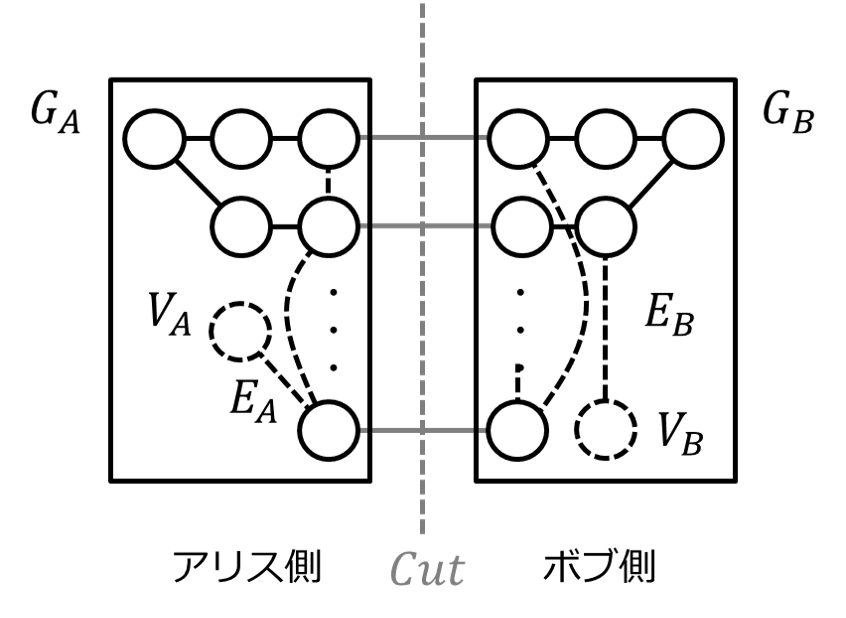
\includegraphics[width=120mm]{Gxy.png}
\end{center}
\caption{$G^{x, y} = (V', E')$}
\label{Gxy}
\end{figure}
構成した下界グラフ$G^{x, y} = (V', E')$に関して,以下の定理が成り立つ.
\begin{theorem}
$G^{x,y}$および$I^{x,y}$を
$k$を交叉判定インスタンスのビット数,$|\mathit{Cut}|$を$G^{x, y}$におけるカット辺のサイズとする.
このとき,任意の$x, y \in \{0, 1\}^k$に対して入力インスタンス$(G^{x, y}, I^{x,y})$が述語$P$を満たすかどうかを判定する{\CONGEST}モデル上の任意のアルゴリズムは
$\Omega (k / |\mathit{Cut}| \cdot \log n)$ラウンドの下界を持つ.
\label{lower}
\end{theorem}
\begin{prf*}
$\mathcal{A}$を,述語$P$を満たすかどうかを判定する分散アルゴリズムであるとする.
アリスとボブは,入力グラフ上での$\mathcal{A}$の実行をシミュレートすることで,
$(x, y)$に対する交差判定問題を解くことができることを示す.
まず最初に,アリスは$G_{A}$のトポロジおよびそこに含まれる頂点のラベリングを,ボブは$G_{B}$のトポロジおよびそこに含まれるのラベリングを構成する.下界グラフが満たす条件より,この構成はアリスとボブの間で通信を行うことなく局所的に計算可能である.構成結果より,アリス,ボブは互いに$V_A$および$V_B$中の頂点の初期状態を知ることが可能である.この初期状態から始まる$A$の実行をシミュレートするために,アリス及びボブはシミュレーションの実行においてカット辺$C$を通じて伝送されるメッセージを互いにやり取りする.
$G_{A}$中の辺で送信されるメッセージ,あるいは$G_{B}$中の辺で送信されるメッセージは,
アリスとボブがそれぞれお互いの通信なしに計算できるため,それとカット辺
$\mathit{Cut}$を通じて送信されるメッセージを互いに受信できれば,$G^{x,y}$全体での$\mathcal{A}$のシミュレーションを(アリスとボブが手分けして)実行することができる.
今アルゴリズム$\mathcal{A}$が$r$ラウンドで終了するとすると,
アリスとボブは上述のシミュレーションにより述語$P$の判定結果を知ることが可能であり,それに必要な通信ビット数は,各辺がラウンドあたり$O(\log n)$ビットの情報を伝送可能であることより,$O(r \cdot |\mathit{Cut}| \cdot \log n)$ビットである.
下界グラフの構成より,述語$P$の真偽と$x$,$y$が交差しているかどうかの真偽は同じであるため,このシミュレーションは$O(r \cdot |\mathit{Cut}| \cdot \log n)$ビットの通信量で交差判定$(x,y)$を解いている.定理~\ref{thm:disjointness}より,この通信量は$\Omega(k)$であり,これより$r = \Omega (k / |\mathit{Cut}| \cdot \log n)$の下界を得ることができる.
\qed
\end{prf*}

\chapter{1-MIS検証問題の$O(1)$ラウンドアルゴリズム}
この章では,1-MIS検証問題を$O(1)$ラウンドで解くアルゴリズムついて述べる.本章のアルゴリズムの結果は,\cite{tanaka2019self}おいて示されている手法と同様のアイデアを{\CONGEST}モデル向けに書き換えただけものであるが,論文の完結性のために本稿においてもアルゴリズムおよび正当性を示しておく.
{\CONGEST}モデルにおいて,入力としてグラフ$G$と独立集合$I$が与えられたとき,
1-MIS検証問題を解くために次のようなアルゴリズム$\mathcal{A}$を実行する.
\begin{enumerate}
\item 各頂点$v \in I$は,自分のIDである$v$.idを隣接頂点全員に送信する.
\item 各頂点$u \notin I$のうち,2種類以上のIDをもらった頂点は0を返し,アルゴリズムから離脱する.
\item 離脱しなかった頂点$u \notin I$のうち,1種類だけのID($v$.idとする)を受信した頂点は
離脱していない全隣接頂点へ$v$.idを送信する.
頂点$u \notin I$は,自身が持つ$v$.idと違う$v$.idが書かれたメッセージは無視し,
自身が持つ$v$.idと同じ$v$.idが書かれたメッセージの数を記憶し,それを$u.a$とする.
\item 各頂点$v \in I$は,自身と同じ$v$.idを返信してきた頂点の集合($v.X$とする)を記憶する.
その後サイズ$|v.X|$を$v.X$中の頂点に送信し,0を返す.
\item メッセージを受け取った$v.X$中の頂点$u$は,送られたサイズ$|v.X| - 1$と$u.a$を比較する.
$|v.X | - 1 = u.a$であれば頂点$u$は$0$を返し,そうでなければ$u$は1を返す.
\end{enumerate}

アルゴリズム$\mathcal{A}$の各ステップは明らかに$O(1)$ラウンドで{\CONGEST}モデルで実装できる.
アルゴリズム$\mathcal{A}$について,以下の定理が成り立つ.
\begin{theorem}
アルゴリズム$\mathcal{A}$は1-MIS検証問題を解くことができる.
\end{theorem}
\begin{prf*}
アルゴリズム$\mathcal{A}$は与えられた入力に対して誤った答えを返すとする.
このとき以下の2つのうち,どちらかが成り立つ. 
\begin{enumerate}
\item 与えられた独立集合が1-MISであり,アルゴリズム$\mathcal{A}$が1-MISでないと返す. 
\item 与えられた独立集合が1-MISでなく,アルゴリズム$\mathcal{A}$が1-MISであると返す. 
\end{enumerate}
アルゴリズム$\mathcal{A}$の5番目のステップで$|v.X| - 1$と$a$を比較して,
$v.X$に含まれる任意の頂点$u$で$|v.X| - 1 = u.a$が成り立つとき$v.X$の頂点はクリークを形成している.
これは$v.X$に含まれる頂点$u \notin I$で等号が成立するのは$u$が$v.X \backslash \{u\}$に含まれる
全ての頂点と隣接している場合のみだからである.

1.の場合,アルゴリズム$\mathcal{A}$が1-MISでないと返したということは,ある$v.X$について
その中の頂点$u \notin I$が1を返したということである.
この場合,$v.X$に含まれる頂点で$u$に隣接していない頂点$w$が存在するはずである.
また$u$と$w$に隣接する$I$内の頂点は$v$のみである.従って$v$を$I$から取り除いて
$u$と$w$を$I$に追加することで独立集合を維持しつつサイズを大きくすることができるため
与えられた独立集合は1-MISではないが,これは仮定に矛盾する. 

2.の場合,アルゴリズム$\mathcal{A}$が1-MISであると返したということは,全ての$v.X$について
その中の頂点$u \notin I$が0を返したということである.この場合,全ての$v.X$がクリークを形成している.
従って,$v.X$の中には独立集合に追加できる可能性のある頂点は存在しない.また,2番目のステップで
離脱した頂点も独立集合点に含まれている1頂点を取り除いただけ追加できる可能性はない.
よって,独立集合を維持しつつサイズを大きくするために追加できる頂点は存在しないため
与えられた独立集合は1-MISであるが,これは仮定に矛盾する. 

以上より,アルゴリズム$\mathcal{A}$は与えられた入力に対して正しい答えを返すことができるため,
1-MIS検証問題を解くことができる.\qed
\end{prf*}
\newpage

\chapter{$k$-MIS検証問題の下界}
この章では,$k$-MIS検証問題の下界についての議論を行う.
4.1節では,2-MIS検証問題の下界についての定理とその証明を述べる.
4.2節では,3-MIS検証問題の下界についての定理とその証明を述べる.
4.3節では,$\ell > 0$に対する,$(4\ell + 5)$-MIS検証問題の下界についての定理とその証明を述べる.

\section{2-MIS検証問題の下界}
この節では2-MIS検証問題の下界についての議論を行う.具体的には,次の定理を証明する.
\begin{theorem}
{\CONGEST}モデルにおいて,2-MIS検証問題を解く全てのアルゴリズムは$\tilde{\Omega} (\sqrt{n})$の
通信ラウンド数を必要とする.
\end{theorem}
\begin{prf*}
まず初めにアリスとボブは下界グラフのインスタンス$G^{x,y} = (V^{x,y}, E^{x,y})$, 
$I^{x,y} : V^{x,y} \to \{0, 1\}$を構築する.このインスタンスにおいて,
頂点ラベリング関数$I^{x,y}(v)$は$v$が検証されるべき独立集合に含まれるとき1,そうでないときに0を返す関数とする.
記述の容易さのため,帰着の元となる交差判定問題のビット数を$N^2$とし,
インスタンス$(x, y)$の各ビットは$N\times N$の要素でインデックス付けされているものとする.
$(i, j) \in N \times N$.でインデックス付けされている$x$,$y$のビットを$x_{i,j}$および$y_{i,j}$で表すものとする.
また,$x$,$y$に含まれる1のビットの個数を$|x|$,$|y|$で表すとする.
$G^{x,y}$の頂点集合$V^{x,y}$は以下の通りに定義される.
\begin{align*}
V^{x,y} &= A^{1} \cup A^{2} \cup B^{1} \cup B^{2} \cup C, \quad \quad \text{ここで}\\
&\phantom{=} \quad A^{j} = \{a^{j}_{i} \mid 1\leq i \leq N\} \quad \quad \text{($j \in \{1, 2\}$)}, \\
&\phantom{=} \quad B^{j} = \{a^{j}_{i} \mid 1\leq i \leq N\} \quad \quad \text{($j \in \{1, 2\}$)}, \\
&\phantom{=} \quad C = \{c_{i,j} \mid y_{i,j} = 1\}.
\end{align*}
アリス及びボブがシミュレーションする頂点集合$V^{x,y}_{A}$および$V^{x,y}_{B}$はそれぞれ
$V^{x,y}_{A} = A^{1} \cup A^{2}$,$V^{x,y}_{B} = B^{1} \cup B^{2} \cup C$と定める.
$G^{x,y}$の辺集合$E^{x,y}$は以下のように定める.
\begin{align*}
E^{x,y} &= E^{1} \cup E^{2} \cup E_{A} \cup E_{B} \cup E_{C}, \quad \quad \text{ここで}\\
&\phantom{=} \quad E^{j} = \{(a^{j}_{i}, b^{j}_{i}) \mid 1\leq i \leq N\} \quad \quad \text{($j \in \{1, 2\}$)}, \\
&\phantom{=} \quad E_{A} = \{(a^{1}_{i},a^{2}_{j}) \mid x_{i,j}=0\}, \\
&\phantom{=} \quad E_{B} = \{(c_{i,j},b^{1}_{i}) \mid y_{i,j}=1\} \cup \{(c_{i,j},b^{2}_{j}) \mid y_{i,j}=1\}, \\
&\phantom{=} \quad E_{C} = \{(c_{i,j}, c_{i',j'}) \mid y_{i,j}=y_{i',j'}=1\} \quad \quad \text{($(i, j) \neq (i', j')$)}.
\end{align*}
$C$中の頂点はクリークを成している.
アリス及びボブがシミュレーションする辺集合$E^{x,y}_A$および$E^{x,y}_B$とカット辺の集合$\mathit{Cut}$はそれぞれ
$E^{x,y}_{A} = E_{A}$,$E^{x,y}_{B} = E_{B} \cup E_{C}$,$\mathit{Cut} = E^{1} \cup E^{2}$と定める.
独立集合に含まれる頂点を示すラベリング$I^{x,y}$は以下のように定める.
\begin{align*}
I^{x,y}(v) &= 0 \quad if \quad v \in A^{j} \cup C \quad \quad \text{($j \in \{1, 2\}$)}, \\
I^{x,y}(v) &= 1 \quad if \quad v \in B^{j} \quad \quad \text{($j \in \{1, 2\}$)}.
\end{align*}
グラフ$G^{x, y} = (V^{x,y}, E^{x,y})$を図 \ref{2_G(x,y)}に示す.
図中の頂点のうち灰色のものは独立集合に含まれる頂点を表す.

\begin{figure}[ht]
\begin{center}
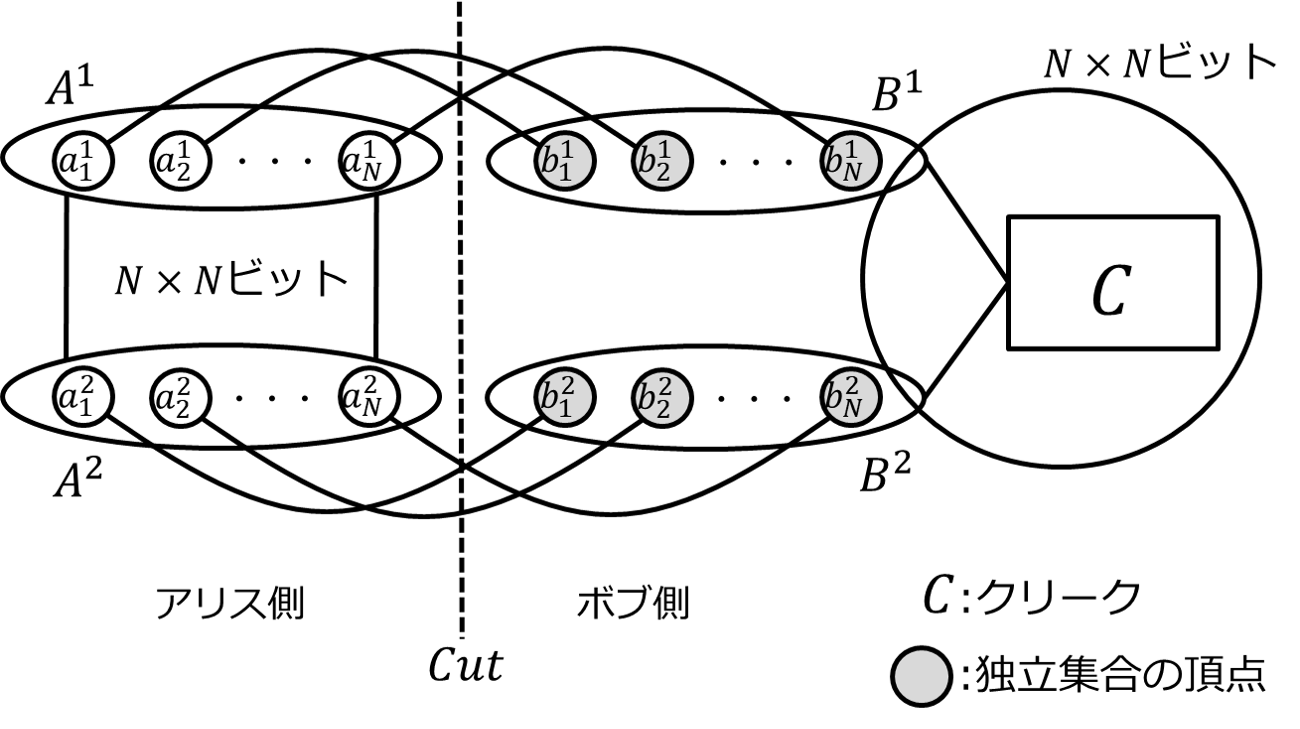
\includegraphics[width=120mm]{2_Gxy.png}
\end{center}
\caption{$G^{x, y} = (V^{x,y}, E^{x,y})$}
\label{2_G(x,y)}
\end{figure}

グラフ$G^{x, y} = (V^{x,y}, E^{x,y})$は,「「$\mathrm{DISJ}_{N \times N} (x, y) = 1$のとき,かつその時に限り$I^{x,y}$が
2-MISでない」」という特性を満たす.これを示すために,次の2点を確認する. \\
(i)$\mathrm{DISJ}_{N \times N} (x, y) = 1$のとき,$I^{x,y}$が2-MISでない: 
$x_{i, j} = y_{i, j} =1$とすると,$b_{i}^{1}$と$b_{j}^{2}$の2点を取り除いて$a_{i}^{1}$, $a_{j}^{2}$, $c_{i, j}$の
3点を追加できることから確認できる. \\
(ii)$\mathrm{DISJ}_{N \times N} (x, y) = 0$のとき,$I^{x,y}$が2-MISである: 
グラフに与えられている独立集合が2-MISでないと仮定する.このとき,ある2点を取り除くことで独立集合に追加できる3点が存在する.
2点の取り除き方は(1)$b_{i}^{1}$と$b_{j}^{1}(i \neq j)$, (2)$b_{i}^{2}$と$b_{j}^{2}(i \neq j)$, (3)$b_{i}^{1}$と$b_{j}^{2}$が考えられる.
(1)では$a_{i}^{1}$と$a_{j}^{1}$の2点しか追加できる可能性がなく,(2)では$a_{i}^{2}$と$a_{j}^{2}$の2点しか追加できる可能性がない.
(3)において,$b_{i}^{1}$を取り除いて$a_{i}^{1}$を追加し,$b_{j}^{2}$を取り除いて$a_{j}^{2}$を追加し,さらに$c_{i, j}$を追加することを考える.
$a_{i}^{1}$と$a_{j}^{2}$が両方とも追加できるのは$x_{i, j} = 1$のときのみであり,$c_{i, j}$が追加できる($c_{i, j}$が存在する)のは
$y_{i, j} = 1$のときのみであるが,これは$\mathrm{DISJ}_{N \times N} (x, y) = 0$に矛盾する.
したがってグラフに与えられている独立集合から2点取り除いて3点追加することはできないため,この独立集合は2-MISである.

今回,$N \times N$ビットの交叉判定インスタンスをグラフに埋め込んでおり,
カット辺のサイズ$|\mathit{Cut}| = 2N$であることが分かる.
{\CONGEST}モデルにおいてグラフ上に与えられた独立集合が2-MISであるかどうかを$r$ラウンドで判定する
アルゴリズム$\mathcal{A}$が存在したとすると,定理\ref{lower}より$\mathcal{A}$は少なくとも
$r = \Omega (N \times N/ 2N \cdot \log n) = \tilde{\Omega}(N)$ラウンド動く.図\ref{2_G(x,y)}から分かる通り,
$A^{1}, A^{2}, B^{1}, B^{2}$はそれぞれ$N$頂点で構成されており,$C$の頂点数は$O(N^{2})$であるため,
グラフ全体の頂点数$n$は$n = O(N + N^{2})$である.したがって$N = \Omega(\sqrt{n})$になるため,
$\tilde{\Omega}(\sqrt{n})$ラウンドの下界を得ることができる. \qed
\end{prf*}
\newpage

\section{3-MIS検証問題の下界}
この節では3-MIS検証問題の下界についての議論を行う.具体的には,次の定理を証明する.
\begin{theorem}
{\CONGEST}モデルにおいて,3-MIS検証問題を解く全てのアルゴリズムは
$\tilde{\Omega} (n)$の通信ラウンド数を必要とする.
\end{theorem}
\begin{prf*}
まず初めにアリスとボブは下界グラフのインスタンス$G^{x,y} = (V^{x,y}, E^{x,y})$, 
$I^{x,y} : V^{x,y} \to \{0, 1\}$を構築する.このインスタンスにおいて,
頂点ラベリング関数$I^{x,y}(v)$は$v$が検証されるべき独立集合に含まれるとき1,そうでないときに0を返す関数とする.
記述の容易さのため,帰着の元となる交差判定問題のビット数を$N^2$とし,
インスタンス$(x, y)$の各ビットは$N\times N$の要素でインデックス付けされているものとする.
$(i, j) \in N \times N$.でインデックス付けされている$x$,$y$のビットを$x_{i,j}$および$y_{i,j}$で表すものとする.
また,$x$,$y$に含まれる1のビットの個数を$|x|$,$|y|$で表すとする.
$G^{x,y}$の頂点集合$V^{x,y}$は以下の通りに定義される.
\begin{align*}
V^{x,y} &= A^{1} \cup A^{2} \cup B^{1} \cup B^{2} \cup C^{1} \cup C^{2} \cup \{s\}, \quad \quad \text{ここで}\\
&\phantom{=} \quad A^{j} = \{a^{j}_{i} \mid 1\leq i \leq N\} \quad \quad \text{($j \in \{1, 2\}$)}, \\
&\phantom{=} \quad B^{j} = \{a^{j}_{i} \mid 1\leq i \leq N\} \quad \quad \text{($j \in \{1, 2\}$)}, \\
&\phantom{=} \quad C^{j} = \{a^{j}_{i} \mid 1\leq i \leq N\} \quad \quad \text{($j \in \{1, 2\}$)}.
\end{align*}
アリス及びボブがシミュレーションする頂点集合$V^{x,y}_{A}$および$V^{x,y}_{B}$はそれぞれ
$V^{x,y}_{A} = A^{1} \cup A^{2}$,$V^{x,y}_{B} = B^{1} \cup B^{2} \cup C^{1} \cup C^{2} \cup \{s\}$と定める.
$G^{x,y}$の辺集合$E^{x,y}$は以下のように定める.

\begin{align*}
E^{x,y} &= E^{A^{1}} \cup E^{A^{2}} \cup E^{B^{1}} \cup E^{B^{2}} 
\cup E^{CA} \cup E^{CB} \cup E^{SA} \cup E^{SB} \cup E_{A} \cup E_{B}, \quad \quad \text{ここで}\\
&\phantom{=} \quad E^{A^{h}} = \{(a^{h}_{i}, a^{h}_{j})  \mid i \neq j\} \quad \quad \text{($h \in \{1, 2\}$)}, \\
&\phantom{=} \quad E^{B^{h}} = \{(b^{h}_{i}, b^{h}_{j})  \mid i \neq j\} \quad \quad \text{($h \in \{1, 2\}$)}, \\
&\phantom{=} \quad E^{CA} = \{(a^{1}_{i}, c^{1}_{i}) \mid 1\leq i \leq N\} \cup \{(a^{2}_{i}, c^{2}_{i}) \mid 1\leq i \leq N\}, \\
&\phantom{=} \quad E^{CB} = \{(b^{1}_{i}, c^{1}_{i}) \mid 1\leq i \leq N\} \cup \{(b^{2}_{i}, c^{2}_{i}) \mid 1\leq i \leq N\}, \\
&\phantom{=} \quad E^{SA} = \{(a^{1}_{i}, s) \mid 1\leq i \leq N\} \cup \{(a^{2}_{i}, s) \mid 1\leq i \leq N\}, \\
&\phantom{=} \quad E^{SB} = \{(b^{1}_{i}, s) \mid 1\leq i \leq N\} \cup \{(b^{2}_{i}, s) \mid 1\leq i \leq N\}, \\
&\phantom{=} \quad E_{A} = \{(a^{1}_{i},a^{2}_{j}) \mid x_{i,j}=0\}, \\
&\phantom{=} \quad E_{B} = \{(b^{1}_{i},b^{2}_{j}) \mid y_{i,j}=0\}.
\end{align*}
$A^{1}$,$A^{2}$,$B^{1}$,$B^{2}$中の頂点はクリークを成している.
アリス及びボブがシミュレーションする辺集合$E^{x,y}_A$および$E^{x,y}_B$とカット辺の集合$\mathit{Cut}$はそれぞれ
$E^{x,y}_{A} = E^{A^{1}} \cup E^{A^{2}} \cup E_{A}$,
$E^{x,y}_{B} = E^{B^{1}} \cup E^{B^{2}} \cup E^{CB} \cup E^{SB} \cup E_{B}$,
$\mathit{Cut} = E^{CA} \cup E^{CB}$と定める.
\Izumi{(論文全体をチェックして,$Cut$や$DIST$等をちゃんとmathitコマンドとmathrmコマンドで囲むようにする)}
独立集合に含まれる頂点を示すラベリング$I^{x,y}$は以下のように定める.
\begin{align*}
I^{x,y}(v) &= 0 \quad if \quad v \in A^{j} \cup B^{j} \quad \quad \text{($j \in \{1, 2\}$)}, \\
I^{x,y}(v) &= 1 \quad if \quad v \in C^{j} \cup \{s\} \quad \quad \text{($j \in \{1, 2\}$)}.
\end{align*}
グラフ$G^{x, y} = (V^{x,y}, E^{x,y})$を図 \ref{3_G(x,y)}に示す.
図中の頂点のうち灰色のものは独立集合に含まれる頂点を表す.
\begin{figure}[ht]
\begin{center}
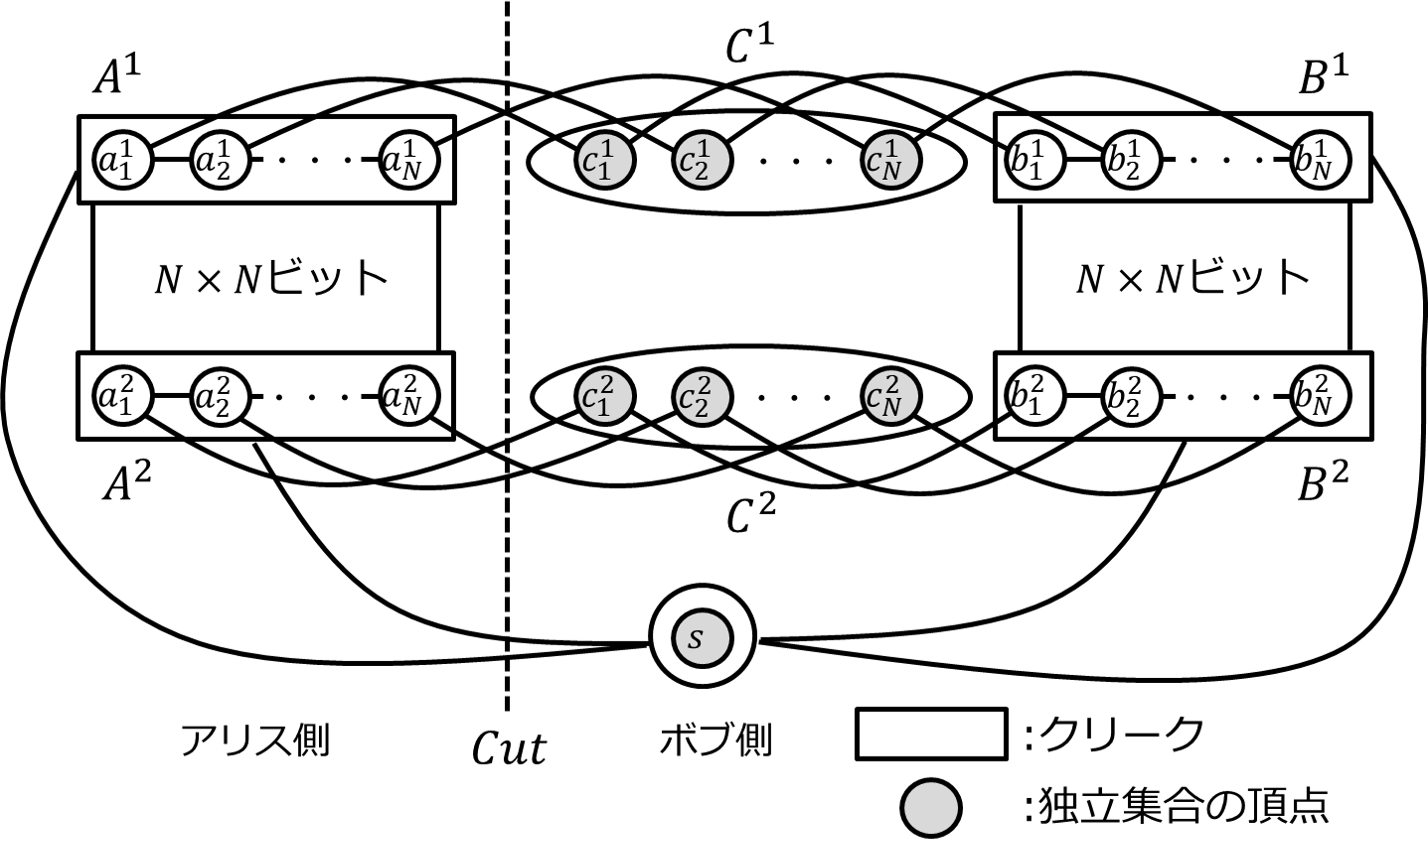
\includegraphics[width=120mm]{3_Gxy.png}
\end{center}
\caption{$G^{x, y} = (V^{x,y}, E^{x,y})$}
\label{3_G(x,y)}
\end{figure}
グラフ$G^{x, y} = (V^{x,y}, E^{x,y})$は,「$\mathrm{DISJ}_{N \times N} (x, y) = 1$のとき,かつその時に限り$I^{x,y}$が
3-MISでない」という特性を満たす.これを示すために,次の2点を確認する. \\
(i)$\mathrm{DISJ}_{N \times N} (x, y) = 1$のとき,$I^{x,y}$が3-MISでない: 
$x_{i, j} = y_{i, j} =1$とすると,$s$と$c_{i}^{1}$と$c_{j}^{2}$の3点を取り除いて
$a_{i}^{1}$, $b_{i}^{1}$, $a_{j}^{2}$, $c_{j}^{2}$の
4点を追加できることから確認できる. \\
(ii)$\mathrm{DISJ}_{N \times N} (x, y) = 0$のとき,$I^{x,y}$が3-MISである: 
グラフに与えられている独立集合が3-MISでないと仮定する.このとき,ある3点を取り除くことで独立集合に追加できる4点が存在するが,
$A^{1}, A^{2}, B^{1}, B^{2}$がそれぞれクリークであるため,4点を追加するためにはそれぞれから1点を選ぶ必要がある.
$c_{i}^{1}$を取り除いて$a_{i}^{1}$と$b_{i}^{1}$を追加し,$c_{j}^{2}$を取り除いて,$a_{j}^{2}$と$b_{j}^{2}$を独立集合に追加したとする.
$a_{i}^{1}$と$a_{j}^{2}$が両方とも追加できるのは$x_{i, j} = 1$のときのみであり,$b_{i}^{1}$と$b_{j}^{2}$が両方とも追加できるのは
$y_{i, j} = 1$のときのみであるが,これは$\mathrm{DISJ}_{N \times N} (x, y) = 0$に矛盾する。したがってグラフに与えられている
独立集合から3点取り除いて4点追加することはできないため,この独立集合は3-MISである.

今回,$N \times N$ビットの交叉判定インスタンスをグラフに埋め込んでおり,
カット辺のサイズ$|\mathit{Cut}| = 4N$であることが分かる.
{\CONGEST}モデルにおいてグラフ上に与えられた独立集合が3-MISであるかどうかを$r$ラウンドで判定する
アルゴリズム$\mathcal{A}$が存在したとすると,定理\ref{lower}より$\mathcal{A}$は少なくとも
$r = \Omega (N \times N/ 4N \cdot \log n) = \tilde{\Omega}(N)$ラウンド動く.図\ref{3_G(x,y)}から分かる通り,
$s$は1頂点,$A^{1}, A^{2}, B^{1}, B^{2}, C^{1}, C^{2}$はそれぞれ$N$頂点で構成されているため,
グラフ全体の頂点数$n$は$n = O(N)$である.
したがって$N = \Omega(n)$になるため,$\tilde{\Omega}(n)$ラウンドの下界を得ることができる. \qed
\end{prf*}
\newpage

\section{$k$-MIS検証問題の下界}
この節では$k$-MIS検証問題の下界についての議論を行う.具体的には,次の定理を証明する.
\begin{theorem}
{\CONGEST}モデルにおいて,任意の$\ell \geq 1$に対して$k = 4\ell + 5$としたとき$k$-MIS検証問題を解く
全てのアルゴリズムは$\Omega\left(n^{2 - \frac{1}{\ell+1}}/\ell \right)$の通信ラウンド数を必要とする.
\end{theorem}

\begin{prf*}
これ以降,$k = 4\ell +5$とする.証明の簡略化のために$N$の$\ell + 1$乗根は整数であると仮定する.このとき$M = \sqrt[\ell + 1]{N}$とする.
また,自然数$i, j, h$が与えられたとき,$\alpha_{i, h}(j)$を$j$を$i$進数で表したときの$h$桁目の値と定義する.
まず初めにアリスとボブは下界グラフのインスタンス$G^{x,y} = (V^{x,y}, E^{x,y})$, 
$I^{x,y} : V^{x,y} \to \{0, 1\}$を構築する.このインスタンスにおいて,
頂点ラベリング関数$I^{x,y}(v)$は$v$が検証されるべき独立集合に含まれるとき1,そうでないときに0を返す関数とする.
記述の容易さのため,帰着の元となる交差判定問題のビット数を$N^2$とし,
インスタンス$(x, y)$の各ビットは$N\times N$の要素でインデックス付けされているものとする.
$(i, j) \in N \times N$.でインデックス付けされている$x$,$y$のビットを$x_{i,j}$および$y_{i,j}$で表すものとする.
また,$x$,$y$に含まれる1のビットの個数を$|x|$,$|y|$で表すとする.
$G^{x,y}$の頂点集合$V^{x,y}$は以下の通りに定義される.
\begin{align*}
V^{x,y} &= A^{h} \cup B^{h}_{j} \cup C^{h}_{j} \cup D^{h}_{j} \cup E^{h}_{j} \cup \{s\} \quad \quad (1\leq j \leq \ell+1, h \in \{1, 2\}) \quad \text{ここで}\\
&\phantom{=} \quad A^{h} = \{a^{h}_{i} \mid 1\leq i \leq N\} \quad \quad \text{($h \in \{1, 2\}$)}, \\
&\phantom{=} \quad B^{h}_{j} = \{b^{h,j}_{i} \mid 1\leq i \leq N,1\leq i \leq \ell+1\} \quad \quad \text{($h \in \{1, 2\}$)}, \\
&\phantom{=} \quad C^{h}_{j} = \{c^{h,j}_{i} \mid 1\leq i \leq M,1\leq i \leq \ell+1\} \quad \quad \text{($h \in \{1, 2\}$)}, \\
&\phantom{=} \quad D^{h}_{j} = \{d^{h,j}_{i} \mid 1\leq i \leq M,1\leq i \leq \ell+1\} \quad \quad \text{($h \in \{1, 2\}$)}, \\
&\phantom{=} \quad E^{h}_{j} = \{e^{h,j}_{i} \mid 1\leq i \leq M,1\leq i \leq \ell+1\} \quad \quad \text{($h \in \{1, 2\}$)}, \\
\end{align*}
アリス及びボブがシミュレーションする頂点集合$V^{x,y}_{A}$および$V^{x,y}_{B}$はそれぞれ
$V^{x,y}_{A} = A^{h} \cup C^{h}_{j} \cup \{s\}$,$V^{x,y}_{B} = B^{h}_{j} \cup D^{h}_{j} \cup E^{h}_{j}$
($1\leq j \leq \ell+1, h \in \{1, 2\}$)と定める.
$G^{x,y}$の辺集合$E^{x,y}$は以下のように定める.

\begin{align*}
E^{x,y} &= E^{A} \cup E^{B} \cup E^{D} \cup E^{SA} \cup E^{AC} 
\cup E^{BE} \cup E^{CD} \cup E^{ED} \cup E_{A} \cup E_{B}, \quad \quad \text{ここで}\\
&\phantom{=} \quad E^{A} = \{(a^{h}_{i}, a^{h}_{i'})  \mid i \neq i'\} \quad \quad \text{($h \in \{1, 2\}$)}, \\
&\phantom{=} \quad E^{B} = \{(b^{h,j}_{i}, b^{h,j}_{i'})  \mid i \neq i'\} \quad \quad \text{($1\leq j \leq \ell+1, h \in \{1, 2\}$)}, \\
&\phantom{=} \quad E^{D} = \{(d^{h,j}_{i}, d^{h,j}_{i'})  \mid i \neq i'\} \quad \quad \text{($1\leq j \leq \ell+1, h \in \{1, 2\}$)}, \\
&\phantom{=} \quad E^{SA} = \{(a^{h}_{i}, s) \mid 1\leq i \leq N\}  \quad \quad \text{($h \in \{1, 2\}$)}, \\
&\phantom{=} \quad E^{AC} = \left\{ \left(a^{h}_{i},c^{h,j}_{\alpha_{M,j}(i-1)+1}\right) \mid 1\leq i \leq N,1\leq j \leq \ell+1\right\} \quad \quad \text{($h \in \{1, 2\}$)}, \\
&\phantom{=} \quad E^{BE} = \left\{ \left(b^{h,g}_{i},c^{h,j}_{\alpha_{M,j}(i-1)+1}\right) \mid 1\leq i \leq N,1\leq g,j \leq \ell+1\right\} \quad \quad \text{($h \in \{1, 2\}$)}, \\
&\phantom{=} \quad E^{CD} = \{(c^{h, j}_{i}, d^{h, j}_{i}) \mid 1\leq i \leq M,1\leq j \leq \ell+1\} \quad \quad \text{($h \in \{1, 2\}$)}, \\
&\phantom{=} \quad E^{ED} = \{(e^{h, j}_{i}, d^{h, j}_{i}) \mid 1\leq i \leq M,1\leq j \leq \ell+1\} \quad \quad \text{($h \in \{1, 2\}$)}, \\
&\phantom{=} \quad E_{A} = \{(a^{1}_{i},a^{2}_{j}) \mid x_{i,j}=0\}, \\
&\phantom{=} \quad E_{B} = \{(b^{1}_{i},b^{2}_{j}) \mid y_{i,j}=0\}.
\end{align*}
$A^{h}$,$B^{h}_{j}$,$D^{h}_{j}$中の頂点はクリークを成している($1\leq j \leq \ell+1, h \in \{1, 2\})$.
アリス及びボブがシミュレーションする辺集合$E^{x,y}_A$および$E^{x,y}_B$とカット辺の集合$\mathit{Cut}$はそれぞれ
$E^{x,y}_{A} = E^{A} \cup E^{SA} \cup E^{AC} \cup E_{A}$,
$E^{x,y}_{B} = E^{B} \cup E^{D} \cup E^{BE} \cup E^{ED} \cup E_{B}$,
$\mathit{Cut} = E^{CD}$と定める.
独立集合に含まれる頂点を示すラベリング$I^{x,y}$は以下のように定める.
\begin{align*}
I^{x,y}(v) &= 0 \quad if \quad v \in A^{h} \cup B^{h}_{j} \cup D^{h}_{j} \quad \quad \text{($1\leq j \leq \ell+1, h \in \{1, 2\}$)}, \\
I^{x,y}(v) &= 1 \quad if \quad v \in C^{h}_{j} \cup E^{h}_{j} \cup \{s\} \quad \quad \text{($1\leq j \leq \ell+1, h \in \{1, 2\}$)}.
\end{align*}
グラフ$G^{x, y} = (V^{x,y}, E^{x,y})$を図 \ref{k_G(x,y)}に示す.
図中の頂点のうち灰色のものは独立集合に含まれる頂点を表す.
\begin{figure}[ht]
\begin{center}
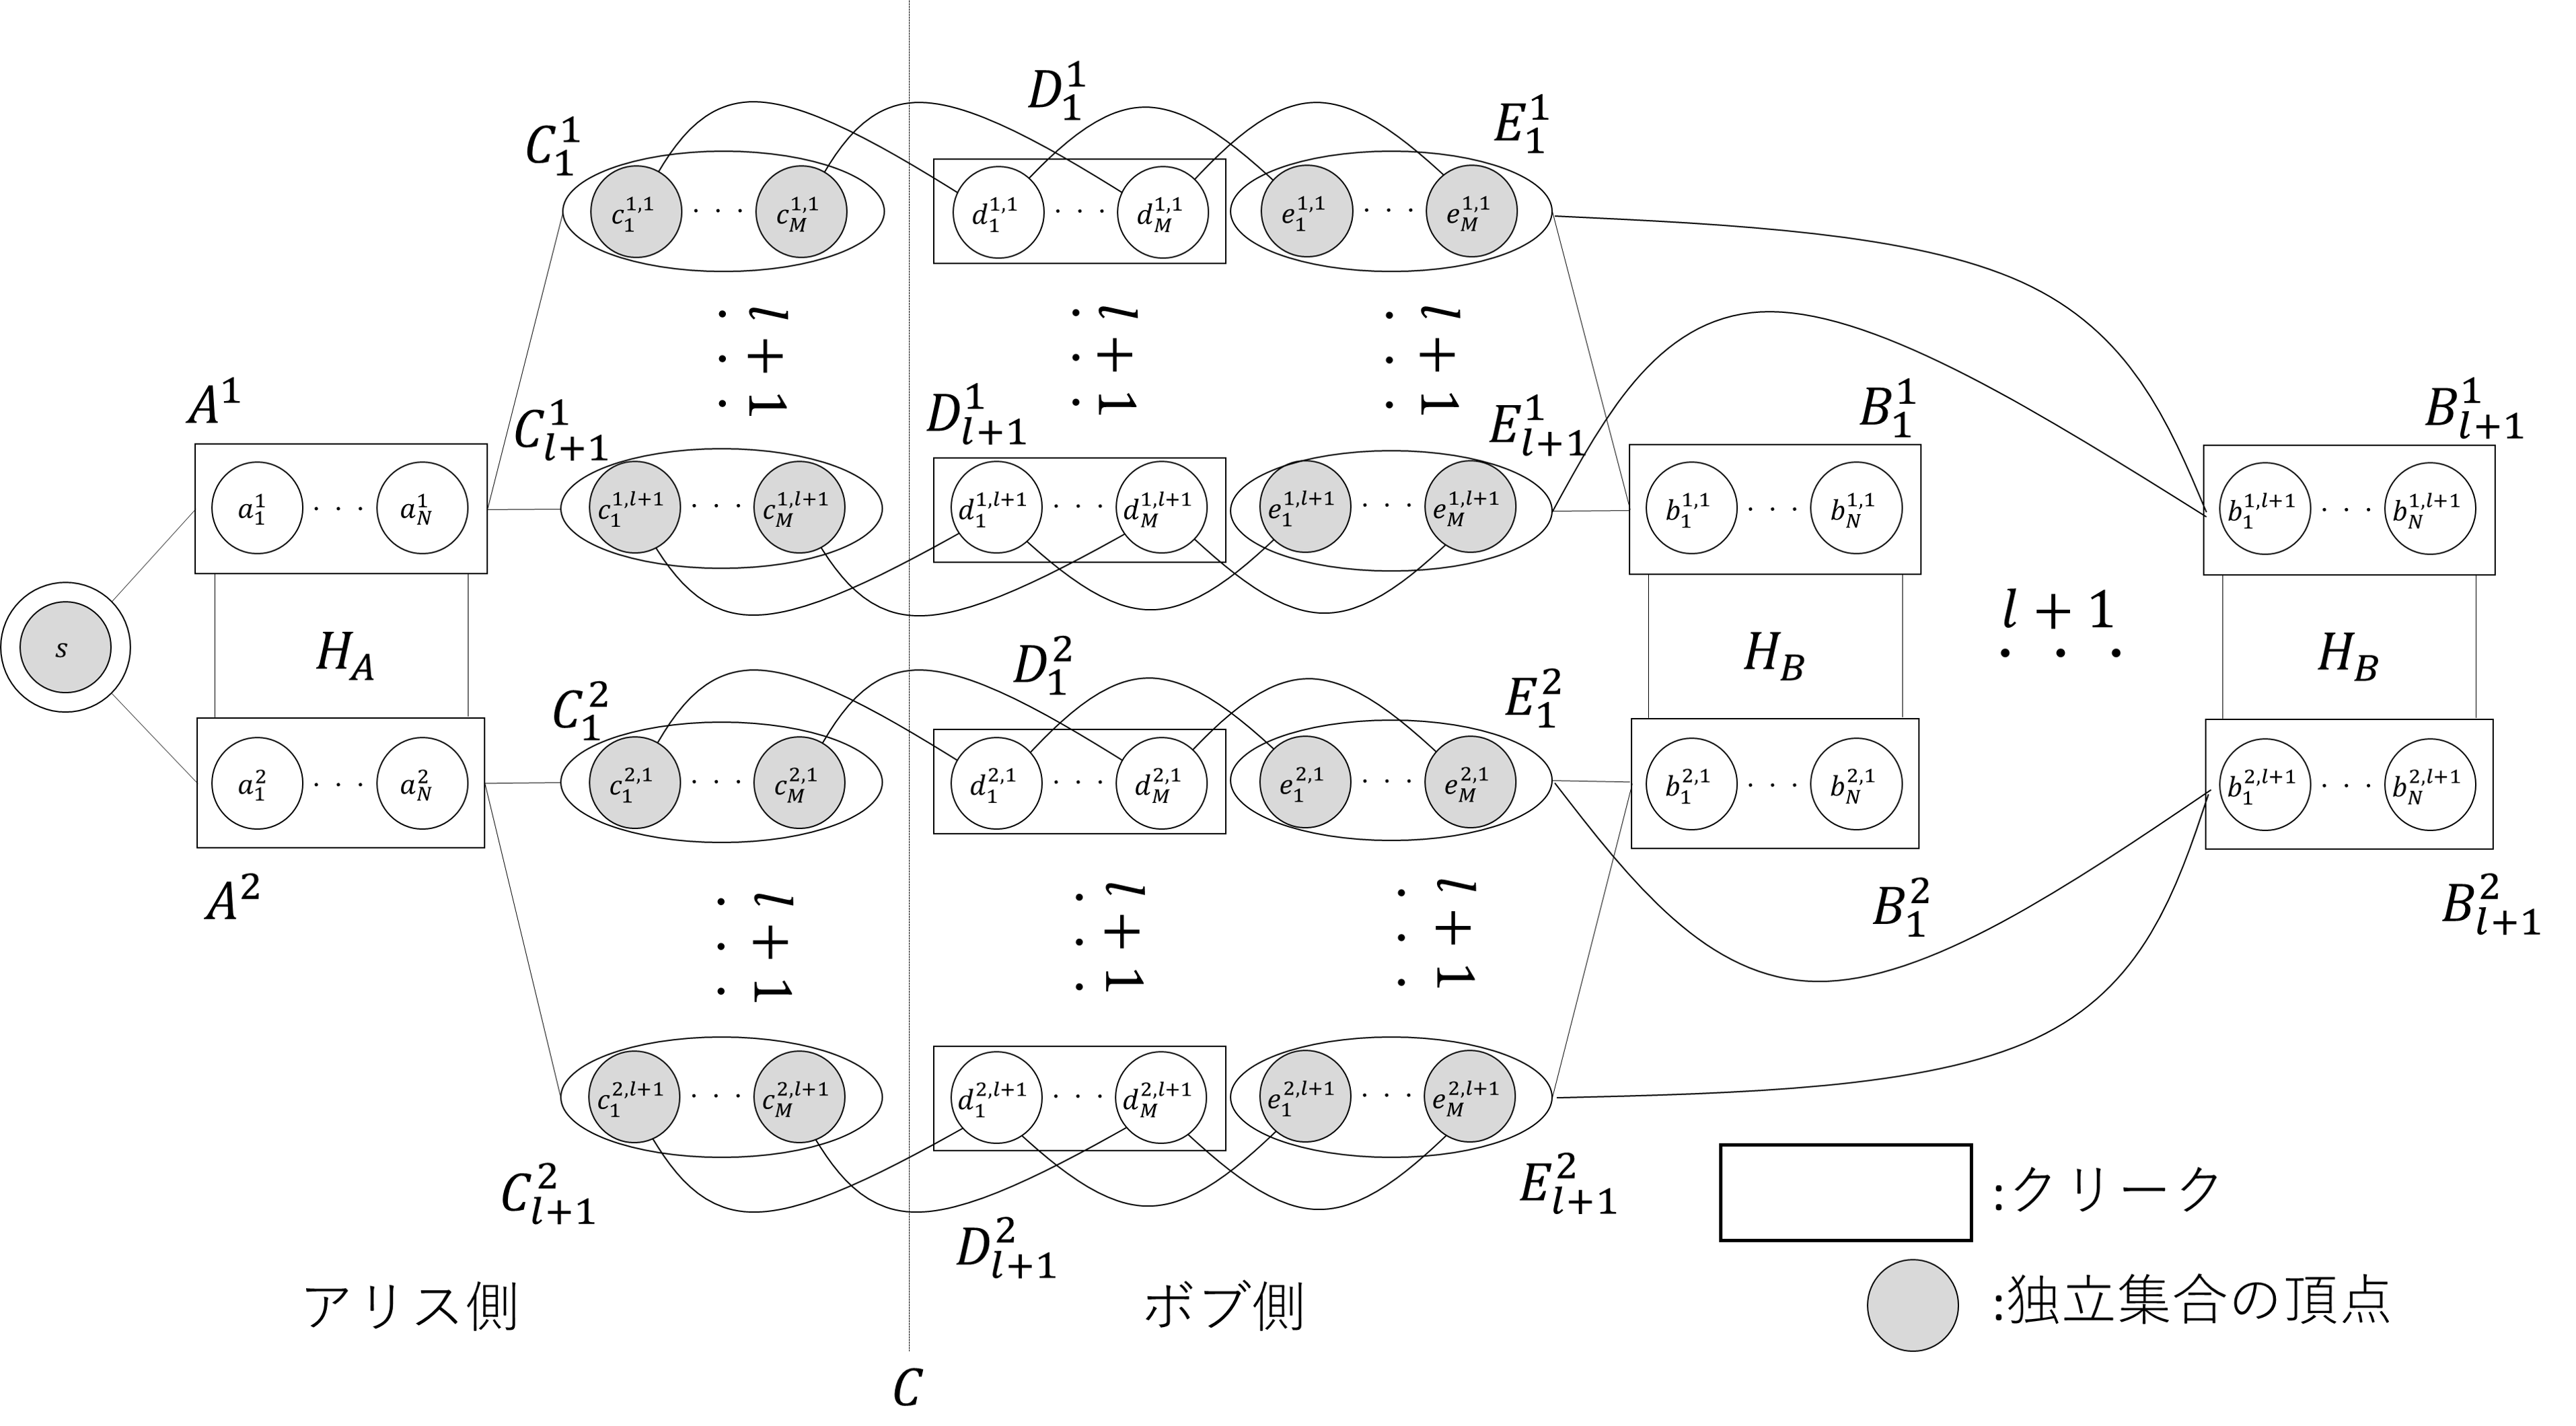
\includegraphics[width=120mm]{k_Gxy.png}
\end{center}
\caption{$G^{x, y} = (V^{x,y}, E^{x,y})$}
\label{k_G(x,y)}
\end{figure}
グラフ$G^{x, y} = (V^{x,y}, E^{x,y})$は,「$\mathrm{DISJ}_{N \times N} (x, y) = 1$のとき,かつその時に限り$I^{x,y}$が
みk-MISでない」という特性を満たす.これを示すために,次の2点を確認する. \\
(i)$\mathrm{DISJ}_{N \times N} (x, y) = 1$のとき,$I^{x,y}$が$k$-MISでない: \\
$x_{i,j}=y_{i,j}=1$であると仮定する.このとき,
\begin{dmath*}
I'=\{s\} \cup \bigcup_{1\leq h \leq \ell+1}c^{1,h}_{\alpha_{M,h}(i-1)+1} \cup 
\bigcup_{1\leq h \leq \ell+1}c^{2,h}_{\alpha_{M,h}(j-1)+1} \cup 
\bigcup_{1\leq h \leq \ell+1}e^{1,h}_{\alpha_{M,h}(i-1)+1} \cup 
\bigcup_{1\leq h \leq \ell+1}e^{2,h}_{\alpha_{M,h}(j-1)+1}
\end{dmath*}
\begin{dmath*}
S=\{a^{1}_{i} \cup a^{2}_{j}\} \cup 
\bigcup_{1\leq h \leq \ell+1}b^{1,h}_{j} \cup 
\bigcup_{1\leq h \leq \ell+1}b^{2,h}_{j} \cup 
\bigcup_{1\leq h \leq \ell+1}d^{1,h}_{\alpha_{M,h}(i-1)+1} \cup  
\bigcup_{1\leq h \leq \ell+1}d^{2,h}_{\alpha_{M,h}(j-1)+1}
\end{dmath*}
とすると
$I \backslash I' \cup S$は独立集合になる.ここで$|I'|=4\ell+5$で$|S|=4\ell+6$であることから,
$k=4\ell+5$に対して$I$は$k$-MISでないことが確認できる. \\
(ii)$\mathrm{DISJ}_{N \times N} (x, y) = 0$のとき,$I^{x,y}$が$k$-MISである: \\ 
グラフに与えられている独立集合が$k$-MISでないと仮定する.このとき,$I'\subseteq I$をサイズ$k$以下の独立集合,
$S\subseteq V\backslash I$を$(I \backslash I') \cup S$が独立集合になるサイズ$|I'|+1$以上の頂点集合とする.
また,$(A^{1}\cup A^{2}) \cap S$を満たす頂点の数を$num(A)$,
$\bigcup_{1\leq i \leq \ell+1}(B_{i}^{1} \cup B_{i}^{2}) \cap S$を満たす頂点の数を$num(B)$,
$\left(\bigcup_{1\leq i \leq \ell+1}C_{i}^{1} \cup \bigcup_{1\leq i \leq \ell+1}C_{i}^{2}\right) \cap S$を
満たす頂点の数を$num(C)$,
$\left(\bigcup_{1\leq i \leq \ell+1}D_{i}^{1} \cup \bigcup_{1\leq i \leq \ell+1}D_{i}^{2}\right) \cap S$を
満たす頂点の数を$num(D)$,\\
$\left(\bigcup_{1\leq i \leq \ell+1}E_{i}^{1} \cup \bigcup_{1\leq i \leq \ell+1}E_{i}^{2}\right) \cap S$を
満たす頂点の数を$num(E)$とする.
任意の$1\leq i \leq M$と$1\leq j \leq \ell+1$に対して$d^{1,j}_{i}$を独立集合に追加するには
$c^{1,j}_{i}$と$e^{1,j}_{i}$を独立集合から取り除く必要がある.
また,任意の$1\leq i \leq M$と$1\leq j \leq l+1$に対して$d^{2,j}_{i}$を独立集合に追加するには
$c^{2,j}_{i}$と$e^{2,j}_{i}$を独立集合から取り除く必要がある.
従って,$num(D)$の値は$num(C)$によって上から抑えられる.
また,$num(D)$の値は$num(E)$によっても上から抑えられる.
任意の$1\leq i \leq N$と$1\leq j \leq \ell+1$に対して,$b^{1,j}_{i}$を独立集合に追加するには,
$\bigcup_{1\leq h \leq \ell+1} e^{1,h}_{\alpha_{M,h}(i-1)+1}$を独立集合から取り除く必要がある.
従って,任意の$1\leq i \leq \ell+1$に対して$B^{1}_{i}$に含まれる頂点を独立集合に追加するには
$\bigcup_{1\leq j \leq \ell+1}E^{1}_{j}$に含まれる頂点を少なくとも$l+1$個独立集合から取り除く必要がある.
同様に任意の$1\leq i \leq N$と$1\leq j \leq \ell+1$に対して,$b^{2,j}_{i}$を独立集合に追加するには,
$\bigcup_{1\leq h \leq \ell+1} e^{1,h}_{\alpha_{M,h}(i-1)+1}$を独立集合から取り除く必要がある.
従って,任意の$1\leq i \leq \ell+1$に対して$B^{2}_{i}$に含まれる頂点を独立集合に追加するには
$\bigcup_{1\leq j \leq \ell+1}E^{2}_{j}$に含まれる頂点を少なくとも$\ell+1$個独立集合から取り除く必要がある.
任意の$1\leq i \leq 2$と$1\leq j \leq \ell+1$に対して,$B^{i}_{j}$はクリークであるので,
$B^{i}_{j}$に含まれる頂点は高々1つしか独立集合に加えることができない.
従って$\bigcup_{1\leq i \leq \ell+1}B^{1}_{i}$から独立集合に加えられる頂点の数は高々$\ell+1$個であり,
$\bigcup_{1\leq i \leq \ell+1}B^{2}_{i}$から独立集合に加えられる頂点の数は高々$\ell+1$個であるので,
$num(B)$の値は$num(E)$の値によって上から抑えられる.
従って$|S|\geq |I'|+1$を満たすには$(num(A) \geq 1$である必要があるが,
$A^{1}$と$A^{2}$はそれぞれクリークあるため$num(A) = 1$もしくは$num(A) = 2$である.\\
はじめに$num(A)=1$の場合を考える.
このとき,$A^{1} \cup A^{2}$に含まれる頂点を独立集合に追加するには頂点$s$を
独立集合から取り除かなければならない.
従って$|I'|=1+num(C)+num(E)$と$|S|=1+num(D)+num(B)$が成り立ち,
$num(C)\geq num(B), num(D)\geq num(E)$より$|I'|\geq |S|$が成り立つがこれは$I'$と$S$の選択に矛盾する.\\
次に$num(A)=2$の場合について考える.
$num(A)=1$の場合と同様に$A^{1} \cup A^{2}$に含まれる頂点を独立集合に追加するには
頂点$s$を独立集合から取り除かなければならない.
従って,$|I'|=1+num(C)+num(E)$と$|S|=2+num(D)+num(B)$が成り立つ.
ここで$|S| \geq |I'|+1$を満たすのは$num(C)=num(D)$かつ$num(B)=num(E)$のときのみである.
また,任意の$1\leq i \leq N$に対して$a^{1}_{i}$を独立集合に追加するには
頂点集合$\bigcup_{1\leq j \leq \ell+1} c^{1,j}_{\alpha_{M,j}(i-1)+1}$を独立集合から取り除く必要がある.
同様に任意の$1\leq i \leq N$に対して$a^{2}_{i}$を独立集合に追加するには
頂点集合$\bigcup_{1\leq j \leq \ell+1} c^{2,j}_{\alpha_{M,j}(i-1)+1}$を独立集合から取り除く必要がある.
従って,$num(C) \geq 2 (\ell+1)$が成り立つ.また,$num(E)\geq num(D)=num(C) \geq 2(\ell+1)$が成り立つ.
ここで,$|I'|\leq k=4\ell+5$であることから,$num(C)=num(E)=2(\ell+1)$となる. \\
$S \cap (A^{1}\cup A^{2})$に含まれる頂点を$a^{1}_{i}$と$a^{2}_{j}$とする.
$a^{1}_{i}$と$a^{2}_{j}$を独立集合に加えるために取り除かれる頂点は
$\{s\} \cup \bigcup_{1\leq h \leq \ell+1} c^{1,h}_{\alpha_{M,h}(i-1)+1} \cup 
\bigcup_{1\leq h \leq \ell+1} c^{2,h}_{\alpha_{M,h}(i-1)+1}$である.
このとき,任意の$\bigcup_{1 \leq i \leq \ell+1}(D^{1}_{i}\cup D^{2}_{i})$に含まれる頂点で
独立集合に含まれる可能性があるのは,
$\bigcup_{1\leq h \leq \ell+1} d^{1,h}_{\alpha_{M,h}(i-1)+1}\cup 
\bigcup_{1\leq h \leq \ell+1} d^{2,h}_{\alpha_{M,h}(i-1)+1}$のみである.
これらの頂点を独立集合に追加するには
$\bigcup_{1\leq h \leq \ell+1} e^{1,h}_{\alpha_{M,h}(i-1)+1}\cup 
\bigcup_{1\leq h \leq \ell+1} e^{2,h}_{\alpha_{M,h}(i-1)+1}$を
独立集合から取り除かなければならない.
このとき,$B^{1}_{1}$と$B^{2}_{1}$で新しく独立集合に加えられる可能性があるのは
$b^{1,1}_{i}$と$b^{2,1}_{j}$だけである.$b^{1,1}_{i}$と$b^{2,1}_{j}$の両方を独立集合に加えられるのは
$b^{1,1}_{i}$と$b^{2,1}_{j}$の間に辺が存在しないときでありこれは$y_{i,j}=1$を意味する.
また,$a^{1}_{i}$と$a^{2}_{j}$が独立集合に含まれることから,$a^{1}_{i}$と$a^{2}_{j}$の間に辺が存在しない.
これは$x_{i,j}=1$を意味するが$\mathrm{DISJ}_{N\times N}(x,y)=0$に矛盾する.

今回,$N \times N$ビットの交叉判定インスタンスをグラフに埋め込んでおり,
カット辺のサイズ$|\mathit{Cut}| = 2(\ell + 1) \cdot M = 2(\ell + 1) \cdot N^{1/(\ell + 1)}$であることが分かる.
{\CONGEST}モデルにおいてグラフ上に与えられた独立集合が$k$-MISであるかどうかを$r$ラウンドで判定する
アルゴリズム$\mathcal{A}$が存在したとすると,定理\ref{lower}より$\mathcal{A}$は少なくとも \\
$r = \Omega \left(N \times N/2(\ell + 1) \cdot N^{1/(\ell + 1)} \cdot \log n\right)=\tilde{\Omega}\left(N^{2 - \frac{1}{\ell + 1}}/\ell \right)$ラウンドで動く.
$s$は1頂点,任意の$1\leq j \leq \ell+1, h \in \{1, 2\})$に対して頂点集合$A^{h}, B^{h}_{j}$はそれぞれ$N$頂点で,
$C^{h}_{j},D^{h}_{j},E^{h}_{j}$の頂点集合はそれぞれ$M=N^{1/(\ell + 1)}$頂点で構成されているため,
グラフ全体の頂点数$n$は$n = O(N)$である.したがって$N = \Omega(n)$になるため,
$\tilde{\Omega}\left(n^{2 - \frac{1}{\ell + 1}}/\ell \right)$ラウンドの下界を得ることができる.
\end{prf*}
\newpage

\chapter{まとめと今後の課題}
\section{まとめ}
本研究では極大独立集合検証問題に対するいくつかの複雑性を示した.
具体的には,1-MIS検証問題に対する$O(1)$ラウンドの上界,
2-MIS検証問題に対する$\tilde{\Omega} (\sqrt{n})$ラウンドの下界,
3-MIS検証問題に対する$\tilde{\Omega} (n)$ラウンドの下界,
$k$-MIS検証問題($k = 4\ell + 5, \ell \geq 1$)に対する$\tilde{\Omega}\left(n^{2 - \frac{1}{\ell + 1}}/\ell \right)$ラウンドの下界を証明した.

\section{今後の課題}
4.3節で一般の$k$に対する$k$-MIS検証問題の下界を証明したが,$k = 4,...,8$については現在
$k=3$同じ下界しか得られていない.この下界をよりタイトにできるかが今後の課題である.
\newpage

\chapter*{謝辞}
本研究の機会を与え,数々の御指導を賜りました泉泰介准教授に深く感謝致します.
また,本研究を進めるにあたり多くの助言を頂き,様々な御協力を頂きました泉研究室
の学生のみなさんに深く感謝致します.

\newpage

\bibliography{M2sato}

\end{document}